\begin{question}[topic=géométrie]
  L'espace est rapporté à un repère orthonormal.

  \begin{enumerate}
    \item Donner un système d'équations paramétriques de la droite $(AB)$
      avec $A : (-1; 2; 3)$ et $B : ((1; -1 ; 1)$.
      \item Le point $C : (2;0;4)$ appartient-il à la droite $(AB)$ ?
    \item Soit $\mathcal{P}$ le plan d'équation $x + y - z - 2  = 0$. Donner
      les coordonnées d'un vecteur normal au plan $\mathcal{P}$. La droite
      $(AB)$ est-elle parallèle au plan $\mathcal{P}$ ?
    \item Quelle est la nature de l'intersection de la droite $(AB)$ et du
      plan $\mathcal{P}$
  \end{enumerate}
\end{question}

\begin{question}[topic=probabilité]
  Les jeunes de 12 à 17 ans représentent 9\% de la population française âgée
  de 12 ans et plus, et 55\% d'entre eux possèdent un smartphone.

  Dans la population française âgée de 12 ans et plus, 34\% des personnes
  agées de plus de 17 ans possèdent un smartphone.

  Pendant une enquête auprès de la population française âgée de 12 ans et
  plus, on choisit une personne au hasard.

  On appelle $J$ l'événement «Être un jeune de 12 à 17 ans parmi la
  population française âgée de 12 ans et plus» et $S$ l'événement «posséder
  un smartphone».

  \begin{enumerate}
    \item Traduire en langage mathématiques les données du texte.
    \item Dans ce texte, lequel des deux événements étudiés est conditionné
      par l'autre ?
    \item Construire et pondérer un arbre de probabilité traduisant la
      situation.
    \item Calculer la probabilité qu'une personne choisie au hasard possède
      un smartphone.
    \item On cherche maintenant à obtenir un arbre pondéré construit dans
      l'autre sens. Construire cet arbre puis présenter les calculs à
      effectuer pour le pondérer.
  \end{enumerate}
\end{question}

\begin{question}[topic=probabilité]
  Le maire de votre commune propose de construire un fontaine à la gloire e
  l'équipe de foot. Le conseil municipal propose un terrain proche du lycée
  de la ville.

  \begin{enumerate}
    \item Un sondage auprès de 100 personnes choisies de façon aléatoire
      indique que 54 personnes sont favorables au projet. Est-ce que ce
      résultat permet d'affirmer que la majorité de la population de la
      ville accepte ce projet ?
    \item Un deuxième sondage est réalisé en interrogeant 600 personnes. On
      constate la même fréquence de votes favorables au projet. Est-ce que
      la conclusion est identique ?
    \item La fréquence de personnes interrogées favorables restant la même,
      déterminer le nombre minimal $n$ de personnes à interroger, pour que
      l'on puisse estimer au seuil de confiance de 95\%, que la majorité de
      la population de la ville est favorable au projet.
  \end{enumerate}
\end{question}

\begin{question}[topic=probabilité]
  En Europe, la proportion de personnes sachant nager est de 65\%

  Dans un lycée de 1543 élèves, il y en a 782 qui savent nager.

  \begin{enumerate}
    \item Déterminer la fréquence de nageurs confirmés dans ce lycée.
    \item Déterminer un intervalle de fluctuation asymptotique au seuil de
      95\%
    \item Peut-on dire que ce lycée est «représentatif» de la proportion de
      nageurs en Europe ?
  \end{enumerate}
\end{question}

\begin{question}[topic=probabilité]
  Dans une entreprise, on produit en grande quantité des pièces de 1 euros.

  On prélève au hasard un pièce. Soit $X$ la variable aléatoire qui, à
  chaque pièce prélèvée associe son diamètre, en millimiètres. On admet que
  la variable aléatoire $X$ suit une loi normale de moyenne \np[mm]{15.5}
  et d'écart-type \np[mm]{0.3}

  \begin{enumerate}
    \item Quelle est la probabilité qu'une pièce tirée au ahsard, ait un
      diamètre compris entre \np[mm]{14.9} et \np[mm]{16.1} ?
    \item Une pièce est déclarée défectueuse si son diamètre est soit
      inférieur à \np[mm]{14.9}, soit supérieur à  \np[mm]{16.1}.
      \begin{enumerate}
        \item Calculer la probabilité qu'une pièce tirée au hasard soit
          défectueuse?
        \item Sachant qu'une pièce n'est pas défectueuse, quelle est la
          probabilité que son diamètre soit inférieur à \np[mm]{15}.
      \end{enumerate}
  \end{enumerate}
\end{question}

\begin{question}[topic=complexes]
  \begin{center}
    \begin{tikzpicture}[scale=0.7]
      \tkzInit[xmin=-6,xmax=6,ymin=-1.5,ymax=8]
      \tkzAxeXY
      \tkzGrid
      \node at (4,3) [draw,circle] {} ;
      \node at (1,7) [draw,circle] {} ;
      \node at (4,3) [below right] { $A$ };
      \node at (1,7) [below right] { $B$ };
    \end{tikzpicture}
  \end{center}
  Dans le plan complexe muni d'un repère orthogonal direct ci-dessus sont
  représentés les points $A$ et $B$.

  \begin{enumerate}
    \item Calculer $\dfrac{z_A}{z_B - z_A}$ en donnant le résultat sous
      forme algébrique puis exponentielle.
    \item Interpréter géométriquement la nature du triangle $OAB$.
    \item Soit $I$ le milieu de $[OB]$. On désigne par $C$ le symétrique de
      $A$ par apport à $I$.

      Quelle est l'affixe du point $C$ ? Préciser la nature du quadrilatère
      $OABC$.
  \end{enumerate}
\end{question}

\begin{question}[topic=exponentielle]
  Soit la fonction $f$ définie sur $[0;+\infty[$ par $f(t) = 8(e^{-t} -
  e^{-2t})$ et soit $\mathcal{C}$ sa courbe représentative dans un
  repère orthogonal.

  Au temps $t = 0$, on injecte un médicament à un animal.

  La concentration sanguine (en $\mathrm{mg.L^{-1}}$) de la substance
  injectée, exprimée en heures, est égale à $f(t)$.

  \begin{enumerate}
    \item Que représentent $f(0)$, $f(\ln 2)$, $f(1)$ ? En donner la valeur
      exacte.
    \item Déterminer la limite de $f$ en $+\infty$
    \item Calculer $f'(0)$.
    \item Au bout de combien de temps la concentration retombera-t-elle à la
      moitié de sa valeur maximale ?

      On donnera une valeur approchée à la minute près.
  \end{enumerate}
\end{question}

\begin{question}[topic=suites]
  Soit la fonction $f$ définie sur $]-2; +\infty[$ par $f(x) =
  \dfrac{4x+1}{x+2}$.

  Soit la suite associée $(u_n)$ définie âr $u_0 = 5$ et pour tout $n$
  entier naturel, $u_{n+1} = f(u_n)$.

  \begin{enumerate}
    \item Soit la courbe représentative de $f$, la droite d'équation $y =
      x$. Placer $u_0, u_1, u_2$ sur l'axe des abscisses.

      \begin{center}
        \begin{tikzpicture}[scale=0.5]
          \tkzInit[xmin=-3,xmax=17,ymin=-4.5,ymax=8]
          \tkzAxeXY
          \tkzGrid
          \draw [thick] plot [smooth,domain=-1:17] (\x , {(4*\x - 1)/(\x +
            2)}) ;
          \draw [very thick] (-3,-3) -- (8,8) ;
        \end{tikzpicture}
      \end{center}
    \item
      \begin{enumerate}
        \item Quelle conjecture peut-on donner sur la monotonie de la suite
          $(u_n)$ et la convergence de la suite $u$ ?
        \item Montrer que $(u_n)$ est décroissante.
        \item Que peut-on en déduire ?
      \end{enumerate}
  \end{enumerate}
\end{question}

\begin{question}[topic=suites]
  Soit la suite $u$ définie sur $\mathbf{N}$ par : $u_n = \dfrac{n}{n^2 +
  1}$.
  \begin{enumerate}
    \item Donner les variations de la suite $(u_n)$.
    \item Déterminer la limite $l$ de la suite $(u_n)$.
    \item L'algorithme ci-dessous permet de déterminer le rang $n$ à prtir
      duquel $\lvert u_n -l \rvert \leqslant 10^{-3}$.

      Compléter cet algorithme.

      \begin{center}
        \begin{tabular}{p{3cm}p{5cm}}
          \textbf{Variables :}  & $n$ est un entier naturel. \\
                                & \\
          \textbf{Traitement :} & Affecter à $n$ la valeur 0 \\
                                & Tant que $\dfrac{n}{n^2 + 1} \geqslant \dots$ \\
                                & \phantom{xx} $\mid$ Affecter à $n$ la valeur … \\
                                & Fin tant que \\
                                & \\
          \textbf{Sortie :}     & Afficher : … \\
        \end{tabular}
      \end{center}
  \end{enumerate}
\end{question}

\begin{question}[topic=logarithme]
  Soit la fonction définie par $f(x) = \ln(x^2 + 2)$ et $I = [ 0 ; +\infty
  [$.

  \begin{enumerate}
    \item Rappeler la dérivée de $\ln(u)$. Calculer la dérivée de $f$ sur
      $I$.

      On pose $g(x) = f(x) - x$.
    \item Étudier les variations de $g$ sur $I$.
    \item Justifier que l'équation $g(x) = 0$ admet une unique solution
      $\alpha$ sur $[1;2]$.
    \item Par un algorithme, ou à la calculatrice, donner un encadrement de
      $\alpha$ d'amplitude $10^{-1}$.
  \end{enumerate}
\end{question}

\begin{question}[topic=lois]
  Une société de matériel informatique se fournit auprès d'une usine de
  composants électroniques. La probabilité que l'un de ces composants
  présente un défaut est de \np{0.02}.

  On admet que le nombre de composants achetés dans l'usine soit suffisament
  important pour que l'achat de 50 composants soit assimilé à 50 tirages
  indépendants avec remise. On appelle $X$ la variable aléatoire associée au
  nombre de composants défectueux dans ce loit.

  \begin{enumerate}
    \item Quel type de loi suit la variable aléatoire $X$ ? Préciser ses
      paramètres.
    \item Quelle est la probabilité qu'exactement 2 des composants achetés
      soient défectueux ?
    \item Quelle est la probabilité qu'au moins un de des composants achetés
      soit défectueux.
    \item Sur chaque lot de 50 composant achetés, quel est le nombre moyen
      de composants défectueux ?
    \item La société commande à présent un lot de 500 composants.

      Elle compte 15 composants défectueux dans ce lot. En utilisant un
      intervalle de fluctuation au seuil de 95\%, dire si la proportion de
      \np{0.02} composants défectueux annoncée par l'usine est fiable.
  \end{enumerate}
\end{question}

\begin{question}[topic=tvi]
  On considère la fonction $f$ définie sur $]0;+\infty[$ par \[ f(x) = \ln x
  + \frac{x^2}2 - 1 . \]

  \begin{enumerate}
    \item Étudier les variations de la fonction $f$ définie sur
      $]0;+\infty[$. On précisera les limites aux borne.
    \item Dresser le tableau de variation de $f$.
    \item Montrer que l'équation $f(x) = 0$ admet une unique solution
      $\alpha$ sur $\mathcal{D}_f$, et justifier le fait que $1 < \alpha <
      2$.
    \item Quel algorithme permettrait d'avoir une valeur approchée à
      $10^{-3}$ près de $\alpha$ ? (on ne demande pas de l'écrire, mais
      juste d'expliquer le principe).
  \end{enumerate}
\end{question}

\begin{question}[topic=suites]
  Soit une suite $(u_n)$ dont aucun terme n'est nul.

  Soit la suite $(v_n)$ définie par : \[ v_n = 1 + \frac{1}{u_n} . \]
  \begin{enumerate}
    \item Montre que si $(u_n)$ est minorée par 1, alors $(v_n)$ est majorée
      par 2.
    \item Dans cette question, on définit plus précisément la suite $(u_n)$
      par : \[ \begin{cases} u_0 = 3 \\ u_{n+1} = \frac{u_n}{u_n = 2}
      \end{cases} . \] Montrer que $(v_n)$ est une suite géométrique de
      raison 2. Quelle est la limite de la suite $(v_n)$ ?
    \item Exprimer $v_n$ en fonction de $n$. En déduire une expression de
      $u_n$ en fonction de $n$, puis la limite de la suite $(u_n)$.
  \end{enumerate}
\end{question}

\begin{question}[topic=suites]
  On considère une suite $(u_n)$.

  L'algorithme ci-dessous permet de calculer le terme $u_n$ pour une valeur
  donnée en entrée.

  \begin{center}
    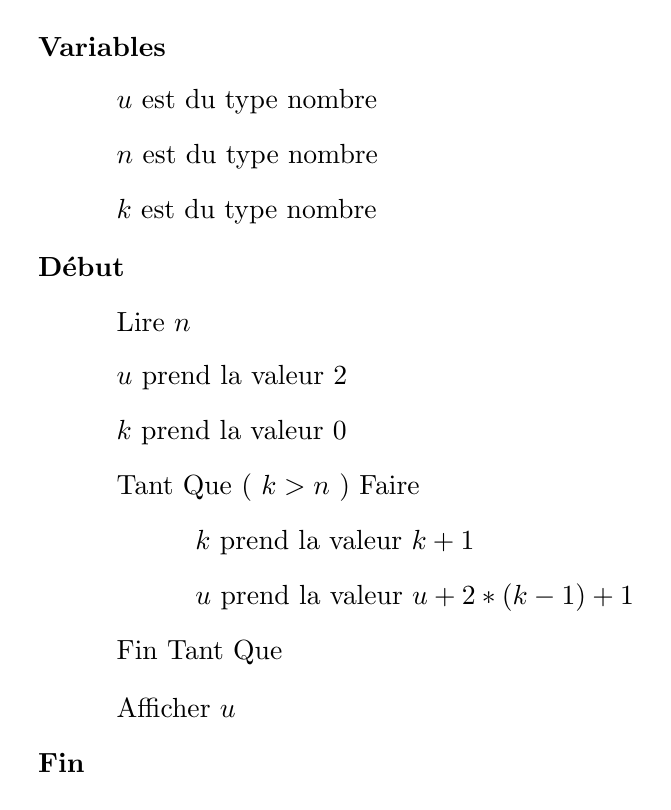
\begin{tikzpicture}[yscale=0.7]
      \draw (0,0) node [anchor=west] { \textbf{Variables} } ;
      \draw (1,-1) node [anchor=west] { $u$ est du type nombre } ;
      \draw (1,-2) node [anchor=west] { $n$ est du type nombre } ;
      \draw (1,-3) node [anchor=west] { $k$ est du type nombre } ;
      \draw (0,-4) node [anchor=west] { \textbf{Début} } ;
      \draw (1,-5) node [anchor=west] { Lire $n$ } ;
      \draw (1,-6) node [anchor=west] { $u$ prend la valeur 2 } ;
      \draw (1,-7) node [anchor=west] { $k$ prend la valeur 0 } ;
      \draw (1,-8) node [anchor=west] { Tant Que ( $ k > n$ ) Faire } ;
      \draw (2,-9) node [anchor=west] { $k$ prend la valeur $k + 1$} ;
      \draw (2,-10) node [anchor=west] { $u$ prend la valeur $u + 2 * (k - 1) + 1 $ } ;
      \draw (1,-11) node [anchor=west] { Fin Tant Que } ;
      \draw (1,-12) node [anchor=west] { Afficher $u$ } ;
      \draw (0,-13) node [anchor=west] { \textbf{Fin} } ;
    \end{tikzpicture}
  \end{center}
  \begin{enumerate}
    \item Les deux propositions suivantes sont-elles \textbf{vraies} ou
      \textbf{fausses} ? Justifier.
      \begin{enumerate}
        \item $u_3 = 11$.
        \item Pour tout $n \in \mathbf{N}, u_{n+1} = u_n + 2n + 1.$
      \end{enumerate}
    \item Montrer que la suite $(u_n)$ est strcitement décroissante.
  \end{enumerate}
\end{question}

\begin{question}[topic=espace]
  L'espace est muni d'un repère orthonormal $(O,\vv{\ivec}, \vv{\jvec},
  \vv{k})$.

  On considère un point $A(1;2;-3)$ et un plan $\mathcal{P}$ d'équation
  cartésienne : $2x - y + z + 1 = 0$.
  \begin{enumerate}
    \item Déterminer les coordonnées d'un vecteur normal au plan
      $\mathcal{P}$.
    \item Déterminer une représentation paramétrique de la droite
      $\mathcal{D}$ passant par le point $A$ et parallèle au plan
      $\mathcal{P}$.
    \item Déterminer les coordonnées du point d'intersection de la droite
      $\mathcal{D}$ et du plan $\mathcal{P}$.
  \end{enumerate}
\end{question}

\begin{question}[topic=espace]
  L'espace est muni d'un repère orthonormal $(O,\vv{\ivec}, \vv{\jvec},
  \vv{k})$.

  On considère les points $A(3;-1;4), B(2;1;4)$ et $C(3;-2;0)$.

  \begin{enumerate}
    \item Montrer que les points $A, B$ et $C$ ne sont pas alignés.
    \item Montrer que les vecteur $\vv{n}\begin{pmatrix} 8 \\ 4 \\ -1
      \end{pmatrix}$ est orthogonal au plan $(ABC)$.
    \item En déduire une équation cartésienne du plan $(ABC)$.
  \end{enumerate}
\end{question}
